\documentclass{fkpset}

\usepackage{tikz-qtree,tikz-qtree-compat}
\usepackage{lscape}
\usepackage{caption}
\captionsetup[figure]{font=Large}
\lfoot{Due Monday, April 29\textsuperscript{th} 2019}
\begin{document}
\vspace{-1.9cm}
\begin{center}
  {\LARGE \scshape Math Forum Reflective Essay} \\[.5em]
  {\Large \scshape Forest Kobayashi}
\end{center}
\vspace{.8cm}

\begin{problem}[Prompt]
  Write a 750-1000 word reflective essay about your growth as a
  speaker in Math Forum. Successful essays will incorporate specific
  examples of lessons learned, together with accompanying allusions to
  your own talks as evidence. Readers of your essay should easily be
  able to sense the extent to which you have been engaged in Math
  Forum.\\

  Please note that the audience for your essay is primarily your
  instructor, but every member of the mathematics faculty should be
  able to read (and enjoy) your essay. Finally, to submit your essay,
  please upload a PDF copy of your essay to your drop box, and please
  name your file lastname-essay.pdf.
\end{problem}
\begin{solution}[Response.]
  \setlength{\parindent}{2em}

  I've really enjoyed my time in Math Forum. I've learned a lot about
  public speaking, managing my verbal/physical tics, and presenting
  technical information in a non-interactive setting. Honestly, I wish
  there were a sequel course --- I'd be really excited to try my hand
  at a full-hour lecture format, or something like it. I guess I could
  always try to start making YouTube videos or something\ldots but
  yeah, anyways, here are some of my big takeaways from the class:
  \begin{enumerate}[label=\arabic*)]
    \item It is much harder for me to present a non-technical topic
      than it is for me to present something like a theorem.
    \item Giving a talk is a vastly different experience from
      presenting material in an interactive setting (e.g.\ tutoring).
      In the latter, you can sometimes rely on your audience to signal
      where you need to slow down, what isn't quite clear, and so on.
      Because talks are more static and non-interactive, you have to
      put in a \emph{lot} of work ahead-of-time to identify places
      where your audience could get lost. As such,
    \item Knowing how to explain a topic well is \emph{not} the same
      thing as knowing how to give a good presentation on it. The
      latter requires a lot more work, including (but not limited to)
      \begin{enumerate}
        \item doing extensive meta-analysis of your own understanding
          of the subject,
        \item compressing that understanding into an easily-digestible
          model that you want to communicate to your audience, and
        \item finding ways to efficiently translate that model to
          words, pictures, and any other medium of communication.
      \end{enumerate}
  \end{enumerate}
  I'll offer some brief thoughts about the first two points, and focus
  the remainder of this essay on the third.
  \section{Why is non-technical exposition harder?}
  I think that one of the biggest challenges to non-technical
  exposition is that things are a lot less discretized. This makes it
  easy to continue packing more and more stuff into your talk, so that
  the audience has an easier time interpolating the underlying
  surface.

  Idea: concepts as $n$-surfaces. Educator: necessarily gives a few
  key points to allow interpolation. Sampling rate ought to be
  proportional to how furrowed the surface is, maybe?

  \section{Why is talk different}

  \section{How to make a talk accessible and/or engaging}


  \begin{figure}[h]
    \centering
    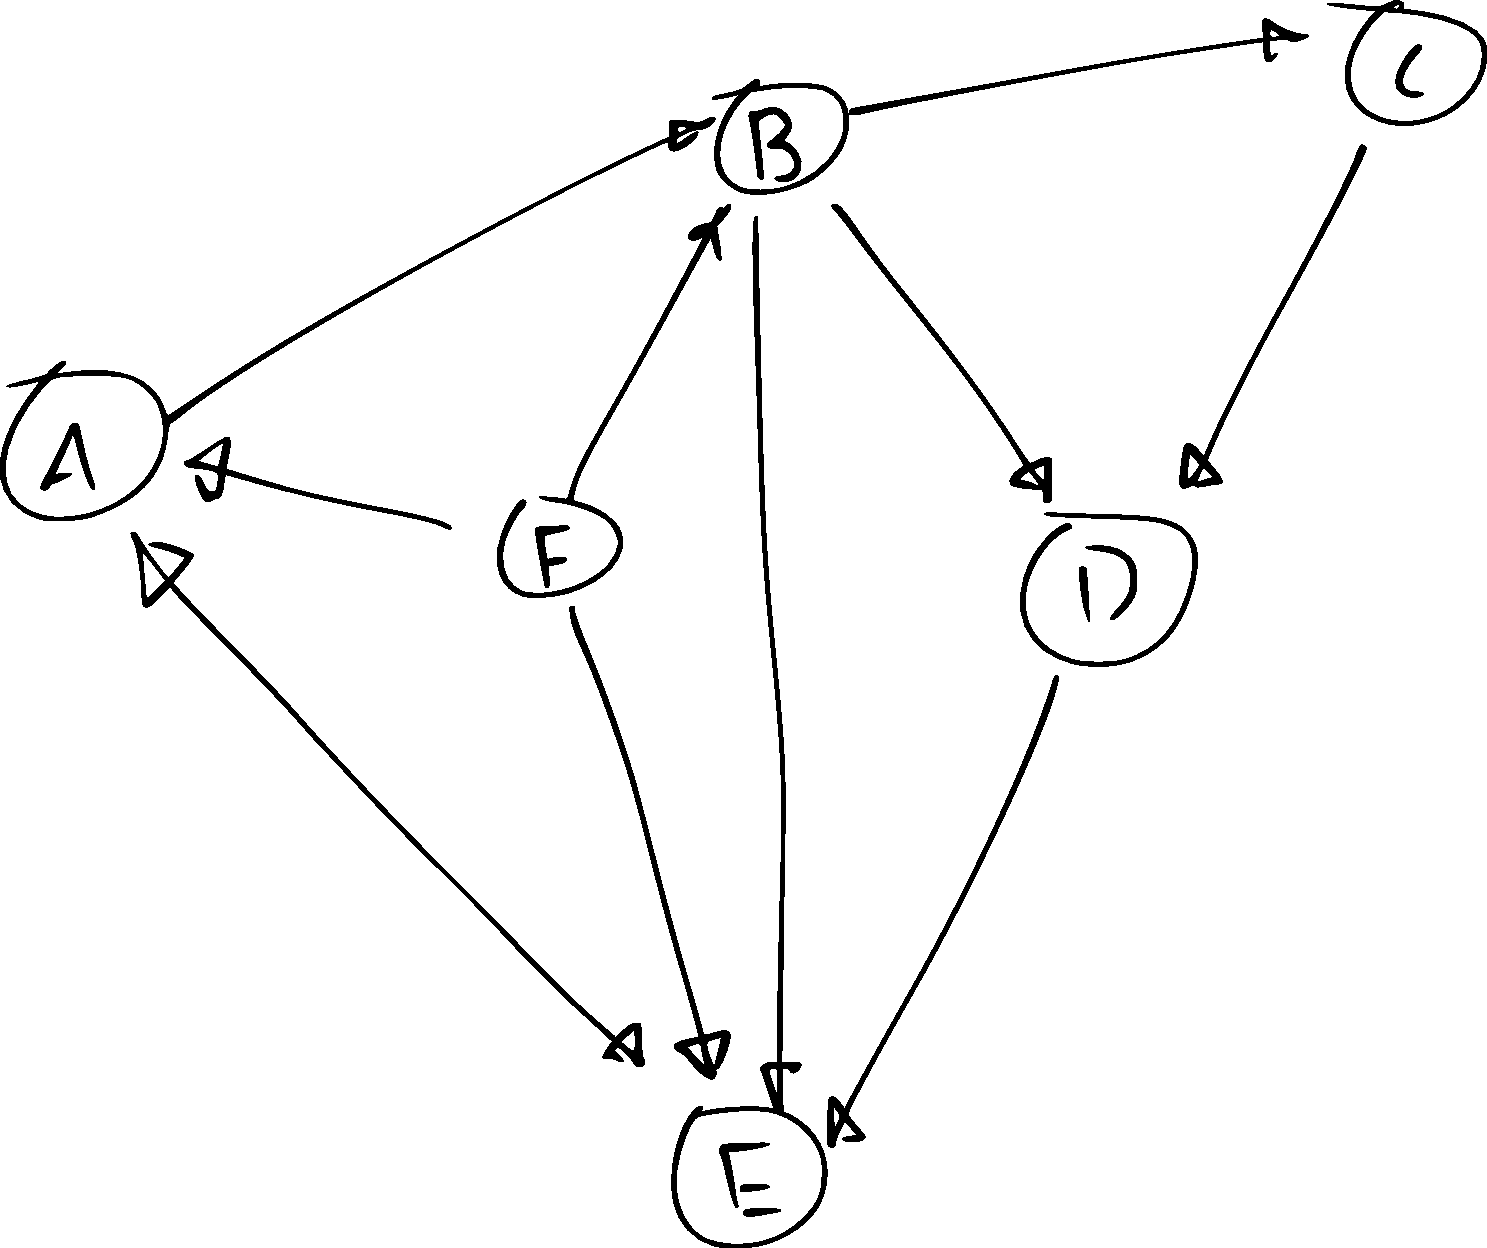
\includegraphics[width=.5\linewidth,keepaspectratio]{graph.pdf}
    \caption{Example of a conceptual digraph}
  \end{figure}

  Key: everything should be justified and motivated. Problem should
  always seem like path of least resistance has been taken. Need to
  \emph{justify} to the audience why we've done stuff.

  The key in a good talk is to focus on polishing the intro and
  conclusion. The technical details are certainly important, but
  provided the audience has a good understanding of the big-picture,
  they'll ultimately be secondary --- with a large-scale perspective,
  audience can reacquire whatever knowledge they need at some point in
  the future.

  Most audiences are surprisingly capable of grappling with abstract
  technical material, provided it's \emph{interesting}. This is what
  you have to focus on. Motivate everything, make everything feel
  gratifying and sensible, and so on.

  Problem is \emph{not} quite ``people aren't great at abstract
  reasoning.'' People do plenty of abstract reasoning --- it's a very
  human thing, in fact. The problem is that abstraction is often
  \emph{uninteresting} to people. Evolutionarily, this would make
  sense, maybe. I really am not an evolutionary psychologist, but I
  imagine that if you were part of a hunter-gatherer society, it
  wouldn't be beneficial to get caught up in ruminations about the
  universe.
  \begin{figure}[h]
    \centering
    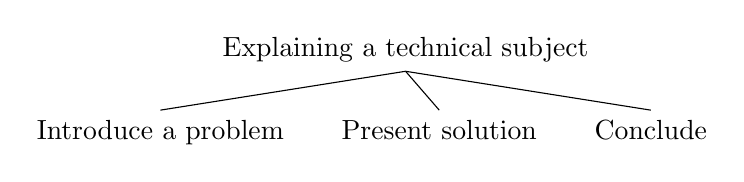
\begin{tikzpicture}[sibling distance=5mm]
      \Tree
      [.{Explaining a technical subject}
        [.{Introduce a problem} ]
        [.{Present solution} ]
        [.{Conclude} ]
      ]
    \end{tikzpicture}
    \caption{Summary of }
  \end{figure}

  \begin{landscape}
    \begin{figure}[p]
      \centering
      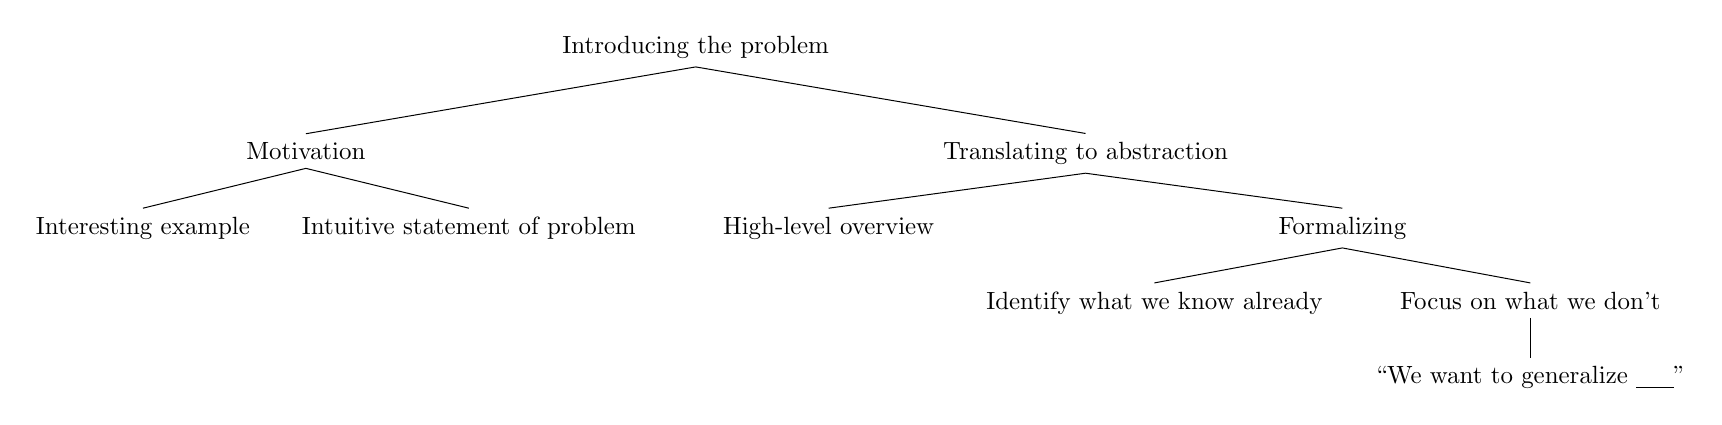
\begin{tikzpicture}[scale=.9, level 1/.style={level distance=1.5cm, sibling distance=10mm}, level 2/.style={sibling distance=5mm}, level 3/.style={sibling distance=5mm}]
        \Tree
        [.{Introducing the problem}
          [.{Motivation}
            [.{Interesting example} ]
            [.{Intuitive statement of problem} ]
          ]
          [.{Translating to abstraction}
            [.{High-level overview} ]
            [.{Formalizing}
              [.{Identify what we know already} ]
              [.{Focus on what we don't }
                [.{``We want to generalize \underline{\phantom{aaa}}''} ]
              ]
            ]
          ]
        ]
      \end{tikzpicture}
      \caption{Introducing a technical subject}
    \end{figure}
  \end{landscape}
  \begin{landscape}
    \begin{figure}[p]
      \centering
      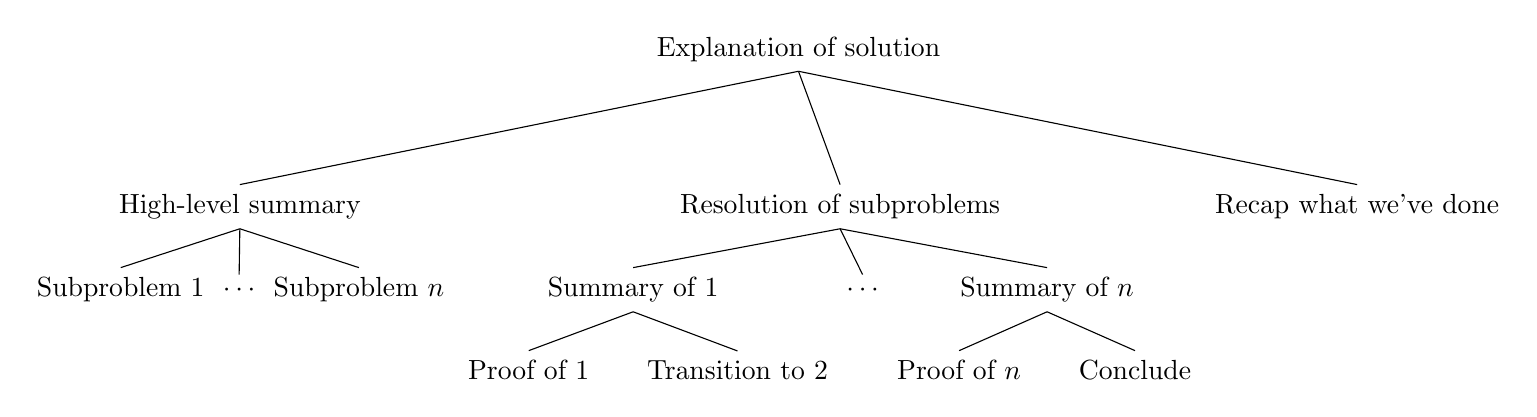
\begin{tikzpicture}[scale=1, level 1/.style={level distance=2cm}, level 2/.style={sibling distance=0mm}, level 3/.style={sibling distance=5mm}]
        \Tree
        [.{Explanation of solution}
          [.{High-level summary}
            [.{Subproblem 1} ]
            [.{$\cdots$} ]
            [.{Subproblem $n$} ]
          ]
          [.{Resolution of subproblems}
            [.{Summary of $1$}
              [.{Proof of 1} ]
              [.{Transition to 2} ]
            ]
            [.{$\cdots$} ]
            [.{Summary of $n$}
              [.{Proof of $n$} ]
              [.{Conclude} ]
            ]
          ]
          [.{Recap what we've done} ]
        ]
      \end{tikzpicture}
      \caption{Explaining the solution}
    \end{figure}
  \end{landscape}
  \begin{landscape}
    \begin{figure}[p]
      \centering
      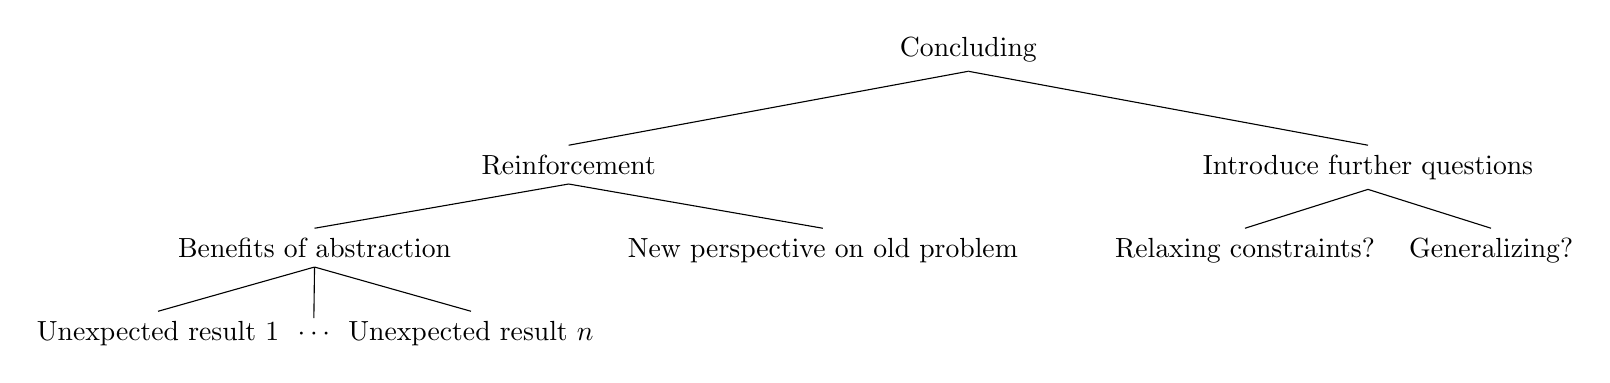
\begin{tikzpicture}[scale=1, level 1/.style={level distance=1.5cm, sibling distance=10mm}, level 2/.style={sibling distance=2mm}, level 3/.style={sibling distance=0mm}]
        \Tree
        [.{Concluding}
          [.{Reinforcement}
            [.{Benefits of abstraction}
              [.{Unexpected result 1} ]
              [.{$\cdots$} ]
              [.{Unexpected result $n$} ]
            ]
            [.{New perspective on old problem} ]
          ]
          [.{Introduce further questions}
            [.{Relaxing constraints?} ]
            [.{Generalizing?} ]
          ]
        ]
      \end{tikzpicture}
      \caption{Wrapping things up}
    \end{figure}
  \end{landscape}
\end{solution}



\end{document}
